\usetikzlibrary{shapes,arrows}
\tikzstyle{block} = [draw, fill=blue!20, rectangle, 
    minimum height=2em, minimum width=4em]
\tikzstyle{circle} = [draw, fill=blue!20, ellipse, 
    minimum height=2em, minimum width=2em]
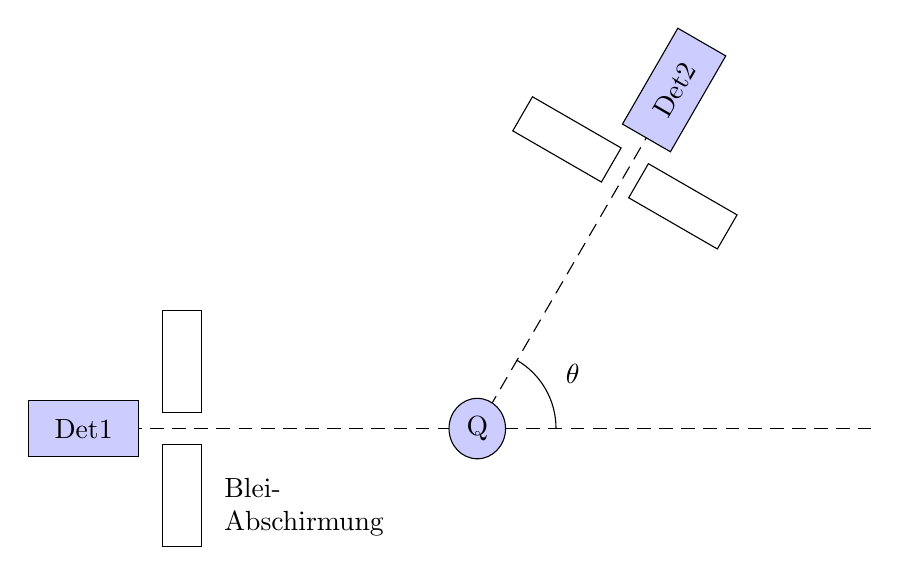
\begin{tikzpicture}
 \coordinate (L) at (-5,0);
 \coordinate (R) at (5,0);
\coordinate (A) at (2.5,4.3);
\coordinate (O) at (0,0);

\draw[dash pattern=on5pt off3pt] (L) -- (R);
\draw[dash pattern=on5pt off3pt] (A) -- (O);
\draw (0.5,0.87) arc (60:0:1);

\node[] at (30:1.4)  {$\theta$};

\node[block, name=det1] at (L) {Det1};
\node[block, name=det2, rotate=60] at (A) {Det2};
\node[circle, name=source] at (O) {Q};

\draw (-4,0.2) rectangle (-3.5,1.5);
\draw (-4,-0.2) rectangle (-3.5,-1.5);

\draw[rotate=60] (4,0.2) rectangle (3.5,1.5);
\draw[rotate=60] (4,-0.2) rectangle (3.5,-1.5);
\node[align=left] at (-2.2,-1) {Blei-\\Abschirmung} ;\end{tikzpicture}